%% LyX 2.3.6 created this file.  For more info, see http://www.lyx.org/.
%% Do not edit unless you really know what you are doing.
\documentclass[12pt,french]{article}
\usepackage{lmodern}
\usepackage{amsmath}
\renewcommand{\familydefault}{\rmdefault}
\usepackage[T1]{fontenc}
\usepackage[utf8]{inputenc}
\usepackage[a4paper]{geometry}
\geometry{verbose,tmargin=2cm,bmargin=2cm,lmargin=2cm,rmargin=2cm}
\usepackage{fancyhdr}
\pagestyle{fancy}
\usepackage{babel}
\makeatletter
\addto\extrasfrench{%
   \providecommand{\og}{\leavevmode\flqq~}%
   \providecommand{\fg}{\ifdim\lastskip>\z@\unskip\fi~\frqq}%
}

\makeatother
\usepackage{booktabs}
\usepackage{url}
\usepackage{amstext}
\usepackage{graphicx}
\usepackage[unicode=true,pdfusetitle,
 bookmarks=true,bookmarksnumbered=false,bookmarksopen=false,
 breaklinks=false,pdfborder={0 0 1},backref=false,colorlinks=false]
 {hyperref}

\makeatletter

%%%%%%%%%%%%%%%%%%%%%%%%%%%%%% LyX specific LaTeX commands.
%% Because html converters don't know tabularnewline
\providecommand{\tabularnewline}{\\}

%%%%%%%%%%%%%%%%%%%%%%%%%%%%%% User specified LaTeX commands.
\usepackage{listings}
\usepackage{xcolor}

\definecolor{codegreen}{rgb}{0,0.6,0}
\definecolor{codegray}{rgb}{0.5,0.5,0.5}
\definecolor{codepurple}{rgb}{0.58,0,0.82}
\definecolor{backcolour}{rgb}{0.95,0.95,0.92}

\lstdefinestyle{mystyle}{
    %backgroundcolor=\color{backcolour},   
    commentstyle=\color{codegreen},
    keywordstyle=\color{magenta},
    numberstyle=\tiny\color{codegray},
    stringstyle=\color{codepurple},
    basicstyle=\ttfamily\footnotesize,
    breakatwhitespace=false,         
    breaklines=true,                 
    captionpos=t,                    
    keepspaces=true,                 
    numbers=left,                    
    numbersep=5pt,                  
    showspaces=false,                
    showstringspaces=false,
    showtabs=false,                  
    tabsize=4
}

\lstset{style=mystyle}

\lstset{
    inputencoding = utf8,  % Input encoding
    extendedchars = true,  % Extended ASCII
    literate      =        % Support additional characters
      {á}{{\'a}}1  {é}{{\'e}}1  {í}{{\'i}}1 {ó}{{\'o}}1  {ú}{{\'u}}1
      {Á}{{\'A}}1  {É}{{\'E}}1  {Í}{{\'I}}1 {Ó}{{\'O}}1  {Ú}{{\'U}}1
      {à}{{\`a}}1  {è}{{\`e}}1  {ì}{{\`i}}1 {ò}{{\`o}}1  {ù}{{\`u}}1
      {À}{{\`A}}1  {È}{{\'E}}1  {Ì}{{\`I}}1 {Ò}{{\`O}}1  {Ù}{{\`U}}1
      {ä}{{\"a}}1  {ë}{{\"e}}1  {ï}{{\"i}}1 {ö}{{\"o}}1  {ü}{{\"u}}1
      {Ä}{{\"A}}1  {Ë}{{\"E}}1  {Ï}{{\"I}}1 {Ö}{{\"O}}1  {Ü}{{\"U}}1
      {â}{{\^a}}1  {ê}{{\^e}}1  {î}{{\^i}}1 {ô}{{\^o}}1  {û}{{\^u}}1
      {Â}{{\^A}}1  {Ê}{{\^E}}1  {Î}{{\^I}}1 {Ô}{{\^O}}1  {Û}{{\^U}}1
      {œ}{{\oe}}1  {Œ}{{\OE}}1  {æ}{{\ae}}1 {Æ}{{\AE}}1  {ß}{{\ss}}1
      {ç}{{\c c}}1 {Ç}{{\c C}}1 {ø}{{\o}}1  {Ø}{{\O}}1   {å}{{\r a}}1
      {Å}{{\r A}}1 {ã}{{\~a}}1  {õ}{{\~o}}1 {Ã}{{\~A}}1  {Õ}{{\~O}}1
      {ñ}{{\~n}}1  {Ñ}{{\~N}}1  {¿}{{?`}}1  {¡}{{!`}}1
      {°}{{\textdegree}}1 {º}{{\textordmasculine}}1 {ª}{{\textordfeminine}}1
      % ¿ and ¡ are not correctly displayed if inconsolata font is used
      % together with the lstlisting environment. Consider typing code in
      % external files and using \lstinputlisting to display them instead.      
  }


\@ifundefined{showcaptionsetup}{}{%
 \PassOptionsToPackage{caption=false}{subfig}}
\usepackage{subfig}
\makeatother

\begin{document}

\lhead{Sorbonne Université, UE LU3PY126 FOAD, 2023}

\rhead{PUJOL Martin}
\title{Projet Dynamique Quantique}
\author{PUJOL Martin}

\maketitle
\tableofcontents{}

\clearpage{}

\section{Introduction}

The ability to describe the time evolution of a quantum system, that is, the evolution over time of its wave function \( \Psi(\vec{r}, t) \), is one of the major results of quantum physics. Quantum mechanics is a fundamental theory of physics that has undergone considerable development in the 20th century, with numerous applications in physics, chemistry, biology, and computer science. Schr\"odinger's equations describe the evolution of quantum systems, and their numerical resolution is a significant challenge in theoretical physics and numerical simulation.

The numerical resolution of the time-dependent Schr\"odinger equations is challenging and requires adapted numerical methods, whether for one-dimensional or multidimensional systems. These methods rely on intensive computation algorithms, which demand substantial computational resources. Computational power, therefore, is a critical resource central to this study.

In this project, we implement numerical methods to solve the time-dependent Schr\"odinger equation for a particle of mass \( m \) subject to the action of a one-dimensional potential \( V(x) \). This equation describes the time evolution of the particle's wave function \( \Psi(x,t) \), given by Equation (3). The one-dimensional potential can be used to model various systems, such as particles in a potential well, electrons in a crystal, atoms in a gas, or molecules in an environment.

First, we study the stationary states of the system, corresponding to time-independent solutions of the Schr\"odinger equation. These stationary states are crucial in quantum physics as they determine the system's fundamental properties, such as energy levels and associated wave functions. To this end, we use the finite difference method to discretize space, replacing partial derivatives with finite differences. We also employ numerical integration methods to compute eigenvalues and eigenvectors of the matrix representing the system's Hamiltonian.

Next, we study the system's time evolution using numerical integration methods, such as Euler's method and the fourth-order Runge-Kutta method (RK4). These methods calculate the wave function \( \Psi(x,t) \) at different times \( t \), using the initial wave function at \( t=0 \) as a starting condition. We also analyze the convergence and stability of these integration methods using numerical analysis techniques.

Finally, we compare numerical results with analytical results for simple systems, allowing us to conclude the importance of spatial and temporal discretization.

\section{Materials and Methods}

\subsection{Resolution Methods: Part 1}

First, we aim to determine the eigenstates of the Hamiltonian. Let us recall its expression:

$$-\frac{\hbar^2}{2m}\frac{d^2\psi}{dx^2} + V(x)\psi = E\psi$$

where $\hbar$ is the reduced Planck constant, $m$ is the particle mass, $V(x)$ is the potential, and $E$ is the eigenvalue associated with the stationary state $\psi$.

We seek to solve this equation to find the eigenvalues of the Hamiltonian. To do so, we discretize the spatial domain using a finite difference method. By discretizing the space, the second derivative is replaced with a centered finite difference, leading to the following equation:

$$-\frac{\hbar^2}{2m}\frac{\psi_{i+1}-2\psi_i+\psi_{i-1}}{\Delta x^2} + V_i\psi_i = E\psi_i$$

where $i$ is the discrete index representing the spatial position along the $x$ direction, and $\Delta x$ is the distance between discrete points. This equation can be rewritten in matrix form as:

$$\mathbf{H}\mathbf{\psi} = E\mathbf{\psi}$$

where $\mathbf{H}$ is the Hamiltonian matrix, $\mathbf{\psi}$ is the discretized wavefunction vector, and $E$ is the discretized eigenvalue.

Using the finite difference method, the matrix $\mathbf{H}$ becomes tridiagonal with specific diagonal and off-diagonal elements. The main diagonal is given by:

$$\mathbf{H}_{ii} = \frac{\hbar^2}{m\Delta x^2} + V_i$$

and the off-diagonal terms are:

$$\mathbf{H}_{i,i+1} = \mathbf{H}_{i+1,i} = -\frac{\hbar^2}{2m\Delta x^2}$$

Next, to find the eigenvalues of the Hamiltonian matrix, we apply a tridiagonal diagonalization method.

This method allows us to diagonalize the Hamiltonian matrix to obtain discrete eigenvalues and their corresponding eigenvectors. These eigenvalues and eigenvectors represent the discrete energy levels and wavefunctions, respectively.

In summary, the finite difference method enables us to discretize the stationary wave equation and find the eigenfunctions of the Hamiltonian in a discrete framework.

\subsection{Resolution Methods: Part 2}

In the second part, we studied the time evolution of the wavefunction of a particle in a one-dimensional potential by solving the time-dependent Schrödinger equation:

$$i\hbar\frac{\partial}{\partial t}\Psi(x,t) = \hat{H}\Psi(x,t)$$

where $\hbar$ is the reduced Planck constant, and $\hat{H}$ is the Hamiltonian operator of the system. To derive a differential relationship for the wavefunction $\Psi(x,t)$, we used the Hamiltonian operator for a particle in a one-dimensional potential:

$$\hat{H} = -\frac{\hbar^2}{2m}\frac{\partial^2}{\partial x^2} + V(x)$$

where $m$ is the particle mass, and $V(x)$ is the one-dimensional potential.

By substituting the Hamiltonian operator into the Schrödinger equation, we obtain:

$$i\hbar\frac{\partial}{\partial t}\Psi(x,t) = -\frac{\hbar^2}{2m}\frac{\partial^2}{\partial x^2}\Psi(x,t) + V(x)\Psi(x,t)$$

We then discretized the spatial domain, replacing the continuous wavefunction with discrete values $\Psi_j^n$, where $j$ represents the spatial position, and $n$ represents the time step. Partial derivatives are replaced with finite differences to derive a recurrence relation for the discrete wavefunction values:

$$i\hbar\frac{\Psi_j^{n+1}-\Psi_j^{n}}{\Delta t} = -\frac{\hbar^2}{2m}\frac{\Psi_{j+1}^{n}-2\Psi_j^{n}+\Psi_{j-1}^{n}}{\Delta x^2} + V_j\Psi_j^{n}$$

where $\Delta x$ and $\Delta t$ are the spatial and temporal discretization steps, respectively, and $V_j$ is the potential value at position $j\Delta x$. This recurrence relation is known as the explicit Euler method for solving the time-dependent Schrödinger equation.

Additionally, we used more precise numerical integration methods, such as the 4th-order Runge-Kutta method (RK4). In this case, a more complex recurrence relation

\subsection{Python Tools}

In this project, various Python libraries were utilized to simulate the dynamics of a Gaussian wave packet in different potentials. First, the NumPy library was employed to manipulate multidimensional arrays, enabling efficient vectorized calculations and optimizing performance.

Next, the Matplotlib library was used for plotting graphs and creating animations. Matplotlib.pyplot was leveraged to plot graphs of the temporal evolution of the wavefunction and the associated particle's mean position. Additionally, Matplotlib.animation was used to create corresponding animations.

The Numba library was also utilized to optimize the performance of calculations.

In summary, these Python libraries allowed for effective and precise simulation of wavefunction dynamics in various potentials, combining code optimization, graphical visualization, and numerical resolution of differential equations.

\subsection{Python Codes (See Appendix)}

The main program for the first part is "resol.py."  
This program solves the wave equation by discretizing space into \(n\) points with a total length \(L\). The `resol` function takes as input the total length \(L\), the number of points \(n\), the potential, and a boolean parameter `Norm` indicating whether the wavefunction should be normalized. The function calculates the eigenvalues `w` and eigenvectors `v` of the tridiagonal matrix associated with the discretized wave equation and returns the results as NumPy arrays. Additionally, the `normalize` function normalizes the eigenvectors if the `Norm` parameter is set to `True`.

The potential functions are stored in the file "potentiels.py."

The script "potentiel stationnaire quantitatif.py" is a Python program designed to evaluate the numerical resolution of the Schrödinger equation for various common potentials and recover the typical results, such as energy quantization and often sinusoidal wavefunctions.

It uses computation and visualization modules, such as Matplotlib, and specific functions to solve the Schrödinger equation for various potentials, including the infinite potential well, potential barrier, double-well potential, periodic potential, and others. The program uses simulation parameters to determine the wavefunctions and energy eigenvalues of the systems. For each potential, it plots the first ten wavefunctions, representing the probability density and the energy eigenvalues of each wavefunction. The results are saved as image files for each potential.

\newline

For the second part, implementing two numerical methods to solve the wavefunction's time evolution was necessary.

The program "euler.py" contains several functions. The primary function, `euler`, implements the Euler method to solve a differential equation. This function takes as input a function `f`, the bounds `a` and `b` of the interval on which the equation is solved, the number \(N\) of discretization steps, the initial condition `y0`, and an optional parameter vector. The function returns an array of \(N\) values taken by \(y\) with a step size \(h\). The Euler method is a simple numerical method for solving differential equations, approximating the function's value at each step \(h\) using its current value and derivative.

The second function in "euler.py" is `normalize`, which normalizes a matrix column-wise by dividing each column by its norm and then divides the matrix by the square root of the discretization step size. This ensures that the sum of the probabilities is equal to 1.

\newline

The second implemented numerical method is the 4th-order Runge-Kutta method. The program "rk4.py" begins by defining a function `rk4`, which takes as input the time step, the function values at time \(t(i)\), a derivative function, and parameters. It returns the new function values for \(t(i+1)\) using the 4th-order Runge-Kutta method.

Next, the program defines a function `RK4`, which takes as input a derivative function, lower and upper bounds \(a\) and \(b\), the number of points \(N\), the function's initial value `y0`, and parameters. It returns an array of \(N\) function values using the 4th-order Runge-Kutta method.

\newline

With these two methods defined, introducing the function that computes the time evolution of a wavefunction becomes essential. The `deriv` function calculates the derivative of the wavefunction `y` using the finite difference method.

\newline

The programs "evolution RK4.py" and "evolution euler.py" evaluate the respective quality of these methods. These programs record some values and plot the evolution of the error on the stationary state for several \(\Delta t\) values. Errors are calculated for \(\Delta t = 1\mathrm{e}{-2}, 1\mathrm{e}{-3},\) and \(1\mathrm{e}{-4}\), and are stored in `error1`, `error2`, and `error3`, respectively. The corresponding times are stored in the arrays `temps1`, `temps2`, and `temps3`.

Finally, the program plots the error evolution for the three \(\Delta t\) values. These graphs are saved as "RK4_Precision.png."

\newline

Finally, several programs were created to highlight the dynamics of a Gaussian wave packet in different potentials. Each of these programs includes an animation and ten graphs tracing the wavefunction's temporal evolution. The graphs also trace the mean position of the particle associated with the wavefunction. This simulation is useful for visualizing and understanding the behavior of wave packets in various potential environments.

Here's the continuation and completion of the translation and enhancement of the text:

```latex
\section{Results}

\subsection{Part One}

\begin{figure}[htbp]
\centering
\begin{minipage}[b]{0.45\linewidth}
\centering
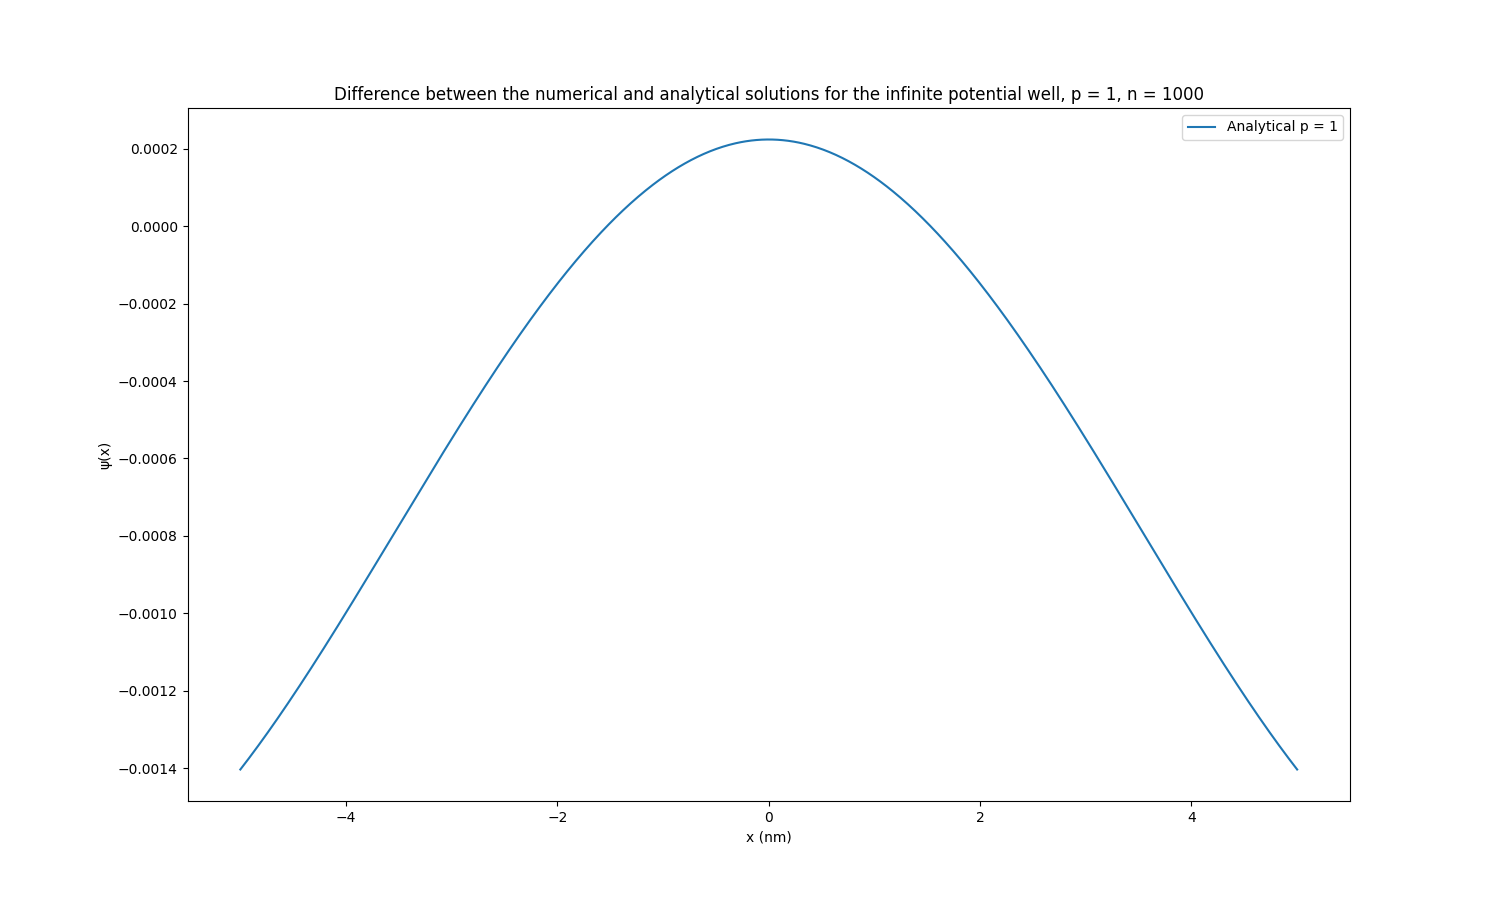
\includegraphics[width=\linewidth]{Partie_I/PartieI_puit_infini_n1000.png}
\caption{Error for $\Delta t = 1\mathrm{e}{-2}$}
\label{fig:infinite-well}
\end{minipage}
\hfill
\begin{minipage}[b]{0.45\linewidth}
\centering
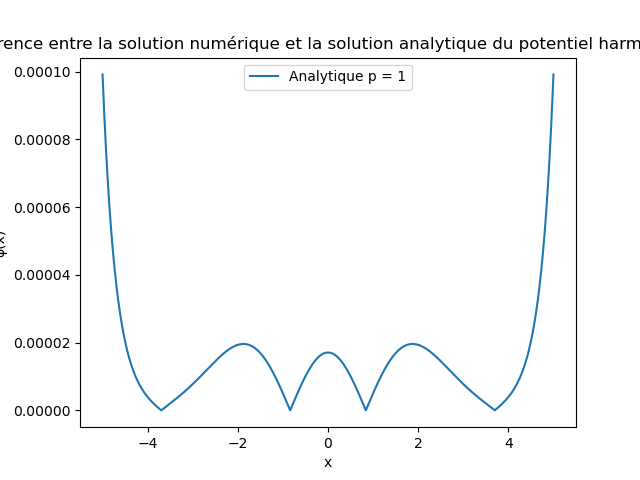
\includegraphics[width=\linewidth]{Partie_I/PartieI_potentiel_harmonique_n10000.png}
\caption{Error for $\Delta t = 1\mathrm{e}{-3}$}
\label{fig:harmonic-potential}
\end{minipage}
\end{figure}

Initially, our objective was to determine the optimal value of \(\Delta t\). While smaller values of \(\Delta t\) are expected to reduce the error, it was equally important to limit the computation time to keep simulations feasible. The graphs above illustrate the error for \(\Delta t\) values of \(1\mathrm{e}{-2}\) and \(1\mathrm{e}{-3}\).

\clearpage

\begin{figure}[htbp]
\centering
\begin{minipage}[b]{0.45\linewidth}
\centering
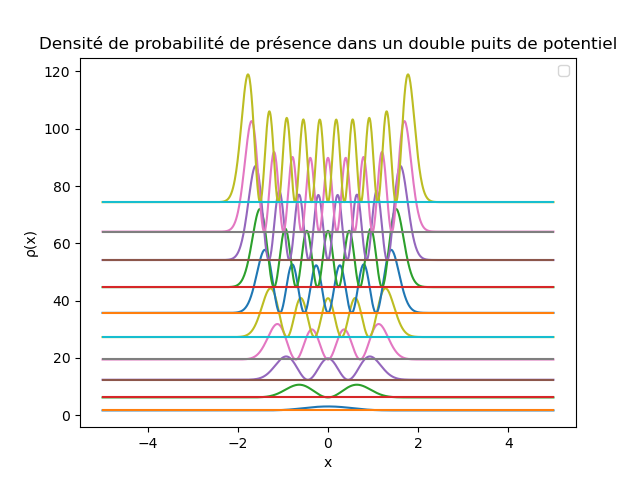
\includegraphics[width=\linewidth]{Partie_I/Double_puits_de_potentiel.png}
\caption{Double-well potential}
\label{fig:double-well}
\end{minipage}
\hfill
\begin{minipage}[b]{0.45\linewidth}
\centering
\includegraphics[width=\linewidth]{Partie_I/Barrière_de_potentiel_amortie.png}
\caption{Damped potential barrier}
\label{fig:damped-barrier}
\end{minipage}
\caption{Wavefunctions for various potentials}
\label{fig:wavefunctions}
\centering
\begin{minipage}[b]{0.45\linewidth}
\centering
\includegraphics[width=\linewidth]{Partie_I/Potentiel_périodique.png}
\caption{Periodic potential}
\label{fig:periodic-potential}
\end{minipage}
\hfill
\begin{minipage}[b]{0.45\linewidth}
\centering
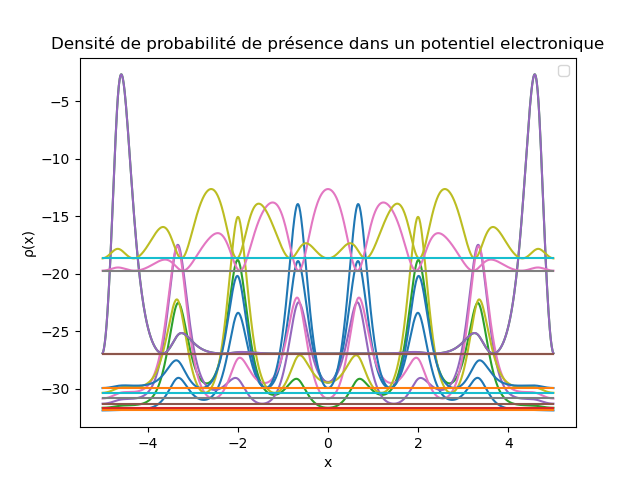
\includegraphics[width=\linewidth]{Partie_I/Potentiel_electronique.png}
\caption{Electronic potential}
\label{fig:electronic-potential}
\end{minipage}
\end{figure}

Figures 3 to 7 illustrate the computed wavefunctions for different potentials, such as double wells, damped potential barriers, periodic potentials, and electronic potentials. The probability densities show highly satisfactory shapes, reminiscent of patterns commonly observed in physics. The results also exhibit the conservation of system symmetry properties and energy level quantization. Each graph depicts ten probability densities, offset by their respective eigenenergies.

\clearpage

\subsection{Part Two}

First, it was necessary to determine the optimal values for \(\Delta t\) and \(\Delta x\) for simulations. To minimize spatial discretization, a minimum value of \(\Delta x = 0.1\) was chosen for a domain of length 10. This limit was essential due to the iterative nature of the calculations. Considering the differential equation, it was expected that the ratio \(\Delta t / (\Delta x)^2\) should not be too large. To confirm this hypothesis, a graph of the error over time was plotted for three different \(\Delta t\) values.

\begin{figure}[htbp]
\centering
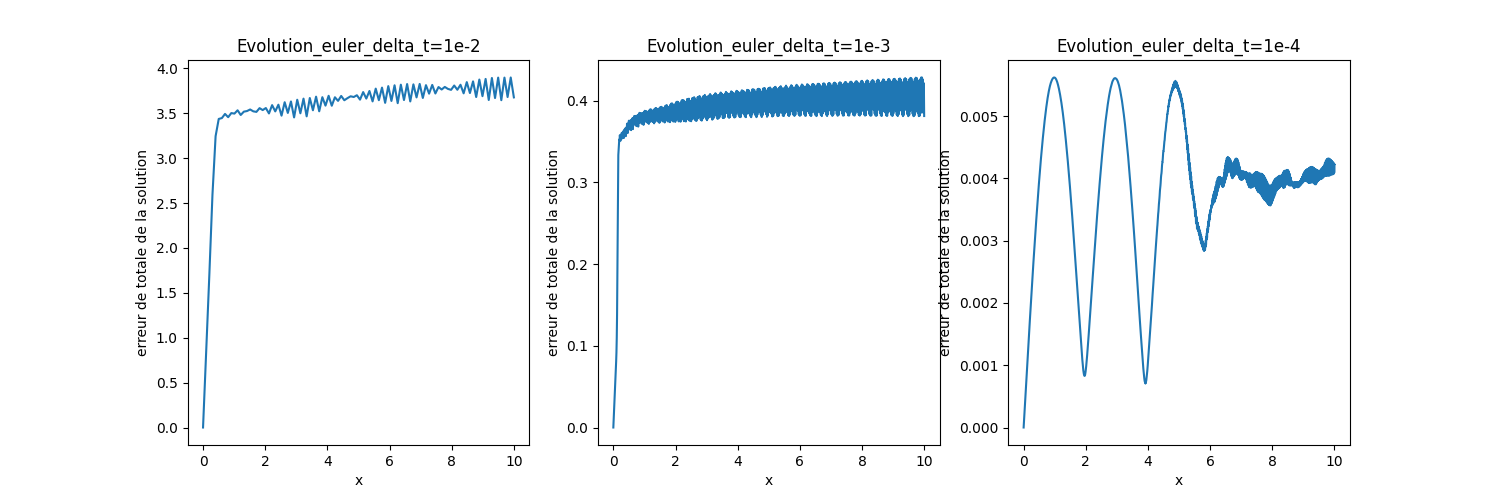
\includegraphics[width=0.7\linewidth]{Partie_II/Euler_Precision.png}
\caption{Error evolution for the Euler method}

\centering
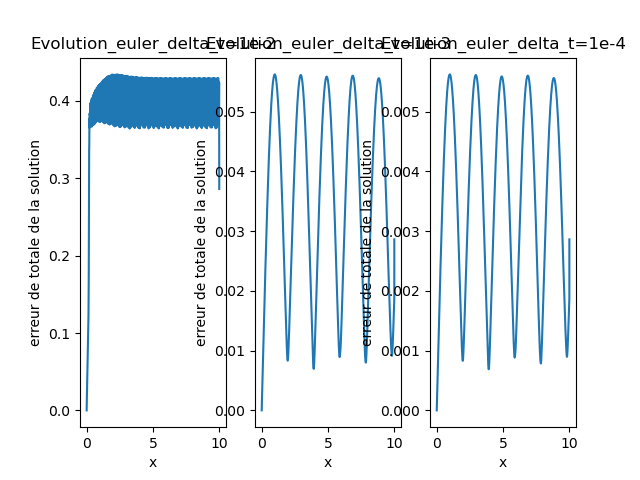
\includegraphics[width=0.7\linewidth]{Partie_II/RK4_Precision.png}
\caption{Error evolution for the Runge-Kutta 4 method}
\end{figure}

The graphs show the error evolution for the Euler method and the Runge-Kutta 4 (RK4) method over time for different \(\Delta t\) values. It can be observed that, for a large \(\Delta t\), the error increases rapidly, whereas for a sufficiently small \(\Delta t\), the error remains low and stable. Overall, the RK4 method is more accurate than the Euler method for all tested \(\Delta t\) values. Therefore, simulations were continued with the RK4 method and \(\Delta t = 1\mathrm{e}{-3}\).

\begin{figure}[htbp]
\centering
\begin{minipage}[b]{0.45\linewidth}
\centering
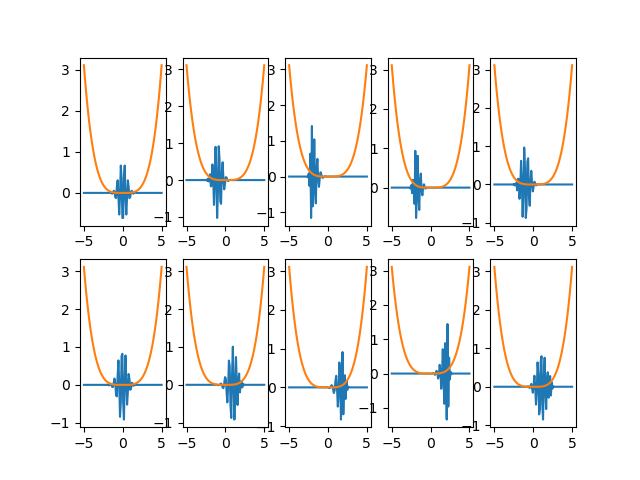
\includegraphics[width=\linewidth]{Partie_II/Dynamique_Paquet_Onde_Potentiel_Harmonique.png}
\caption{Wave packet dynamics in a harmonic potential}
\label{fig:harmonic-dynamics}
\end{minipage}
\hfill
\begin{minipage}[b]{0.45\linewidth}
\centering
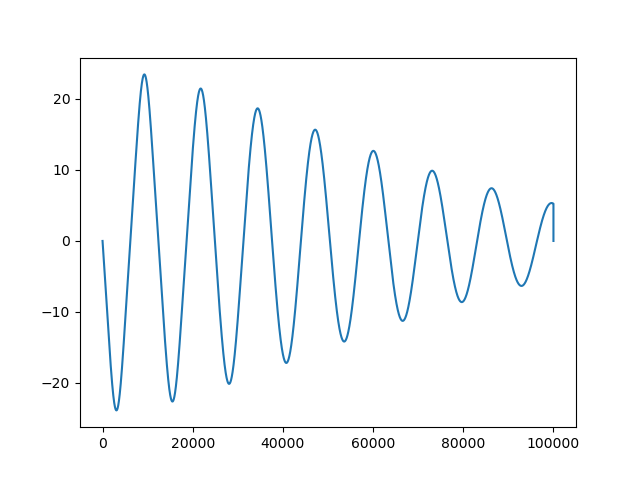
\includegraphics[width=\linewidth]{Partie_II/Position_Moyenne_Paquet_Onde_Potentiel_Harmonique.png}
\caption{Mean position of the particle}
\label{fig:harmonic-mean-position}
\end{minipage}
\end{figure}

Figure 10 shows the oscillation of a wave packet in a harmonic potential. To achieve a significant displacement, the wave packet was assigned very high energy (\(k_0 = 1\mathrm{e}{10}\)). However, despite this high energy, the wave packet's position spreads over time, possibly due to numerical errors. Moreover, the particle's mean position exhibits a periodic oscillation, seemingly converging toward zero. This observation reflects the quasi-classical behavior of the particle in a harmonic potential.

\clearpage

Figures 12 and 13 extend the previous simulations, showing a wave packet traversing a potential field composed of six uniformly spaced electrons. It can be observed that the wave packet appears trapped at the center, where the potential is highest. Figure 13 depicts the same potential as Figure 12 but with higher energy assigned to each electron.

\begin{figure}[htbp]
\centering
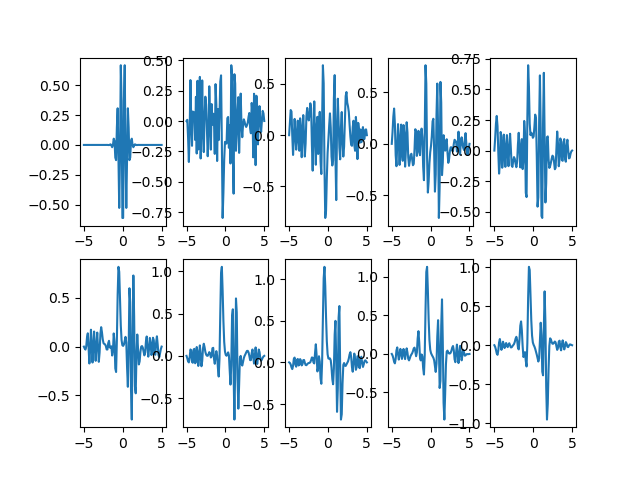
\includegraphics[width=0.5\linewidth]{Partie_II/Dynamique_Paquet_Onde_Potentiel_Electronique_potentiel_plus_bas.png}
\caption{Wave packet dynamics in an electronic potential}
\label{fig:lower-electronic-potential}
\end{figure}

\begin{figure}[htbp]
\centering
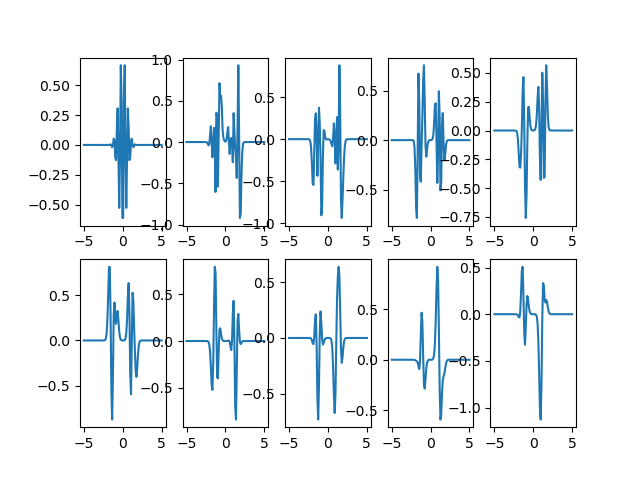
\includegraphics[width=0.5\linewidth]{Partie_II/Dynamique_Paquet_Onde_Potentiel_Electronique.png}
\caption{Wave packet dynamics in a higher electronic potential}
\label{fig:higher-electronic-potential}
\end{figure}

\clearpage

\section{Discussion of Results}

The discussion can be structured into two main parts: numerical methods and observed results.

### Numerical Methods

The first part of the study focused on solving the eigenstates of the Hamiltonian for various potentials. The initial objective was to determine the optimal value of \(\Delta t\) to minimize the error while limiting computation time. Graphs depicting errors for \(\Delta t = 1\mathrm{e}{-2}\) and \(\Delta t = 1\mathrm{e}{-3}\) showed a significant reduction in error for smaller \(\Delta t\) values but at the cost of increased computation time. Thus, \(\Delta t = 1\mathrm{e}{-3}\) was chosen as a reasonable compromise.

The following graphs presented the computed eigenfunctions for various potentials. The resulting probability densities were highly satisfactory, showing patterns consistent with the expected physical properties for each potential, while preserving system symmetry and energy quantization.

In the second part, we examined the temporal evolution of wavefunctions. Optimal \(\Delta t\) and \(\Delta x\) values were determined, ensuring that \(\Delta t / (\Delta x)^2\) remained small. The error evolution graphs for different \(\Delta t\) values validated this approach.

### Observed Results

Regarding the results, it was reassuring to find quantized energy levels and correct analytical solutions for the initial energy levels in the infinite square well and harmonic potential. The shapes of the probability densities were also consistent with expectations. A key confirmation of these calculations was the invariance of wavefunctions over time, in contrast to their linear combinations or wave packets.

Finally, the dynamics of wavefunctions revealed further insights. For example, the periodic oscillation of a Gaussian wave packet in a harmonic potential suggested quasi-classical behavior. Additionally, the trapping of a wave packet by multiple electrons highlighted the quantum mechanical phenomenon of localization.

\section{Conclusion}

This project successfully implemented numerical methods to solve the time-dependent Schrödinger equation based on the system Hamiltonian. The results demonstrated the importance of carefully selecting \(\Delta t\) and \(\Delta x\) to balance accuracy and computational feasibility. The study highlighted the precision of the RK4 method over the Euler method, albeit at a higher computational cost.

The investigation revealed quantized energy levels, consistent analytical predictions, and preserved system symmetry. Additionally, the dynamics of Gaussian wave packets in harmonic and electronic potentials provided valuable insights into quasi-classical behavior and quantum localization.

In summary, the project

 advanced the understanding and application of numerical methods for solving the time-dependent Schrödinger equation, showcasing the quantum properties and dynamics of different systems.

\clearpage

\section{Appendix}

\subsection{Python Codes}

Below are the primary Python scripts used in the project. See the code listing in the respective files:

\lstinputlisting[language=Python,caption={},label {}]{Partie_I/resol.py}
\lstinputlisting[language=Python,caption={},label {}]{Partie_I/potentiels.py}
\lstinputlisting[language=Python,caption={},label {}]{Partie_II/deriv.py}
\lstinputlisting[language=Python,caption={},label {}]{Partie_II/euler.py}
\lstinputlisting[language=Python,caption={},label {}]{Partie_II/rk4.py}
\lstinputlisting[language=Python,caption={},label {}]{Partie_II/evolution_euler.py}
\lstinputlisting[language=Python,caption={},label {}]{Partie_II/evolution_rk4.py}
\lstinputlisting[language=Python,caption={},label {}]{Partie_II/paquet_onde_potentiel_harmonique.py}

\end{document}
